\documentclass[12pt,landscape,letterpaper]{article}
\usepackage{multicol,multirow}
\usepackage{graphicx}
\usepackage{ifthen}
\usepackage[landscape]{geometry}
\usepackage{booktabs}
\usepackage{fontspec}

\setsansfont{Fira Sans}
\setmonofont{Inconsolata}

\makeatother

\ifthenelse{\lengthtest { \paperwidth = 11in}}
    { \geometry{margin=0.4in} }
	{\ifthenelse{ \lengthtest{ \paperwidth = 297mm}}
		{\geometry{top=1cm,left=1cm,right=1cm,bottom=1cm} }
		{\geometry{top=1cm,left=1cm,right=1cm,bottom=1cm} }
	}
\pagestyle{empty}
\makeatletter
\renewcommand{\section}{\@startsection{section}{1}{0mm}%
                                {-4ex plus -.5ex minus -.2ex}%
                                {0.5ex plus .2ex}%x
                                {\sffamily\large}}
\renewcommand{\subsection}{\@startsection{subsection}{2}{0mm}%
                                {-4ex plus -.5ex minus -.2ex}%
                                {0.5ex plus .2ex}%
                                {\sffamily\normalsize\itshape}}

\makeatother
\setcounter{secnumdepth}{0}
\setlength{\parindent}{0pt}
\setlength{\parskip}{0pt plus 0.5ex}
% -----------------------------------------------------------------------
\usepackage{tikz}
\usepackage{float}

\begin{document}
\tikz[remember picture,overlay] \node[opacity=0.1,inner sep=0pt] at (current page.west){
\includegraphics[height=0.8\paperheight]{media/Logo.png}};
\footnotesize

\begin{center}
  {\huge\sffamily\bfseries Betriebsanweisung Matrixtester v1} \\
\end{center}
\setlength{\premulticols}{0pt}
\setlength{\postmulticols}{0pt}
\setlength{\multicolsep}{1pt}
\setlength{\columnsep}{1.8em}
\begin{multicols}{3}

\section{Lieferumfang}
\begin{itemize}
\item Matrixtester
\item USB Type A - Type B Abschlusskabel
\end{itemize}

\section{Inbetriebnahme}
Dieser Abschnitt beschreibt die Inbetriebnahme vor jedem Prüfdurchlauf.

\subsection{\#1 - Anschluss des Gerätes}

Schließen Sie das Gerät mit dem mitgelieferten Anschlusskabel an einer geeigneten USB Schnittstelle an. Alternativ verwenden Sie ein 5V USB Steckernetzteil oder ein 12V Rundsteckernetzteil (nicht im Lieferumfang enthalten).\\

Das Display leuchtet mehrere Sekunden lang blau auf. Anschließend schaltet sich das Display kurz ab und wieder an.\\

Nun zeigt das Display in einer Endlosschleife die Version des Gerätes an und die Aufforderung eine Matrix anzuschließen.\\

\begin{figure}[H]
    \centering
    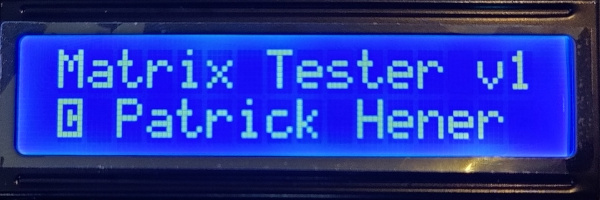
\includegraphics[width=0.2\textwidth]{media/intro-1.jpg}
\end{figure}


\begin{figure}[H]
    \centering
    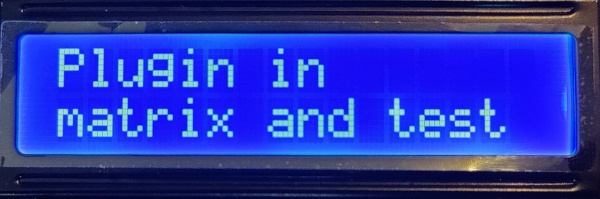
\includegraphics[width=0.2\textwidth]{media/intro-2.jpg}
\end{figure}

\subsection{\#2 Anschluss der Matrix}

Am Matrixtester ist eine Stiftleiste exponiert, die für den Anschluss der Matrix vorgesehen ist. Die Stiftleiste ist mit L (für links) und R (für rechts) auf dem Case des Gerätes beschriftet.\\

Liegt die Matrix, wie nachfolgend abgebildet, so ergibt sich am Stecker die linke und die rechte Seite, wie beschriftet:

\begin{figure}[H]
    \centering
    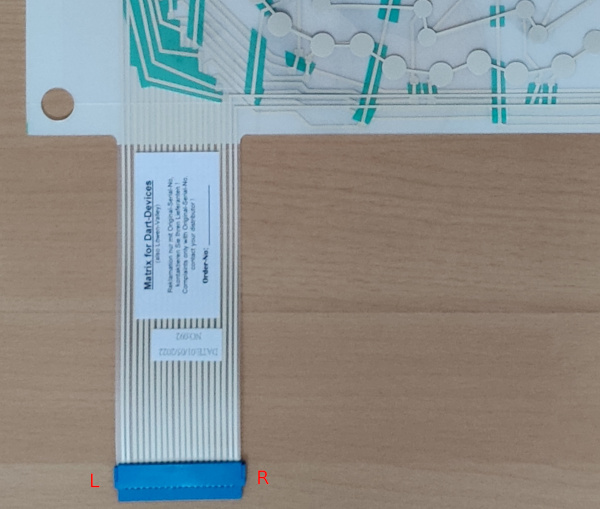
\includegraphics[width=0.2\textwidth]{media/matrix-1.jpg}
\end{figure}

Der Anschluss am Gerät erfolgt demnach wie nachfolgend abgebildet:

\begin{figure}[H]
    \centering
    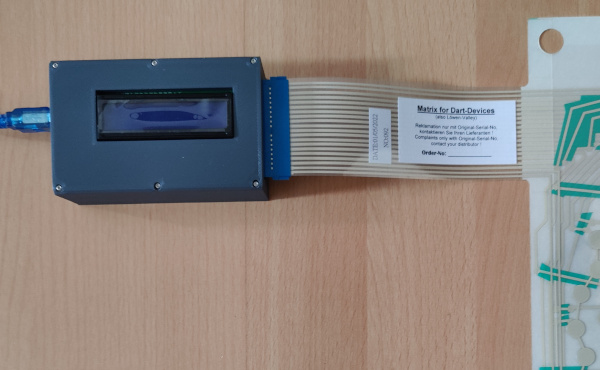
\includegraphics[width=0.2\textwidth]{media/matrix-2.jpg}
\end{figure}

\section{Testen der Matrix}

Für den Start der Erkennung wird ein Kontaktpunkt der Matrix gedrückt und solange gehalten, bis das Display einen Zahlenwert anzeigt:

\begin{figure}[H]
    \centering
    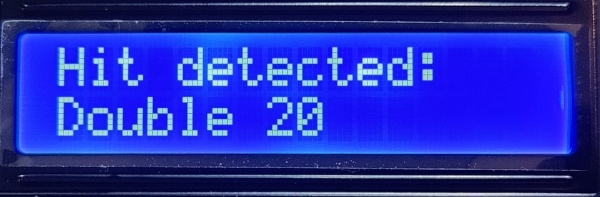
\includegraphics[width=0.2\textwidth]{media/detection-1.jpg}
\end{figure}

Anschließend kann durch einen kurzen Druck auf einen beliebigen Kontaktpunkt der Matrix der nächste Zahlenwert ausgelesen und die Funktion überprüft werden.

\begin{figure}[H]
    \centering
    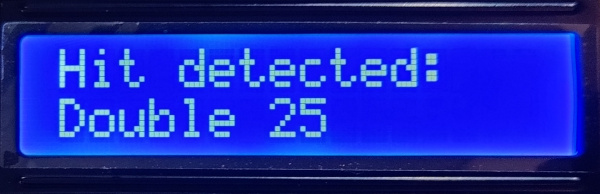
\includegraphics[width=0.2\textwidth]{media/detection-2.jpg}
\end{figure}

Ist die Prüfung der Matrix abgeschlossen kann im laufenden Betrieb die aktuelle Matrix abgesteckt und eine andere Matrix angesteckt werden. Es besteht nicht die Notwendigkeit das Gerät für den Wechsel eine Matrix vom Strom zu trennen.

\vfill
{\hfill
\includegraphics[width=0.9\hsize]{media/Banner.png}\hfill}

\end{multicols}
\end{document}